\documentclass[aspectratio=169,10pt]{beamer}

% Conference deck for the survey paper. Compile from latex/slides/.
\usetheme{metropolis}
\usecolortheme{metropolis}
\usefonttheme{professionalfonts}
\metroset{progressbar=frametitle,numbering=fraction,block=fill,sectionpage=none}
\usepackage[T1]{fontenc}
\usepackage{newtxtext,newtxmath}
\usepackage{graphicx}
\usepackage{booktabs}
\usepackage{array}
\usepackage{tabularx}
\usepackage{amsmath}
\usepackage{tikz}
\usetikzlibrary{positioning,arrows.meta,calc,fit,shadows.blur}
\pdfstringdefDisableCommands{\def\translate#1{#1}}

% Visual system adapted from style_slide_reference.md.
\definecolor{navy}{HTML}{23373B}
\definecolor{blue}{HTML}{2F6268}
\definecolor{blueLite}{HTML}{DCE8E9}
\definecolor{amber}{HTML}{EB811B}
\definecolor{amberLite}{HTML}{FFF0DF}
\definecolor{green}{HTML}{287A63}
\definecolor{greenLite}{HTML}{E3F1EC}
\definecolor{red}{HTML}{B6423C}
\definecolor{redLite}{HTML}{F7E7E5}
\definecolor{ink}{HTML}{233036}
\definecolor{muted}{HTML}{647277}
\definecolor{paper}{HTML}{FFFFFF}
\definecolor{softgray}{HTML}{F2F4F7}

\setbeamercolor{normal text}{fg=ink,bg=paper}
\setbeamercolor{structure}{fg=amber}
\setbeamercolor{frametitle}{fg=navy,bg=paper}
\setbeamercolor{progress bar}{fg=amber,bg=blueLite}
\setbeamercolor{progress bar in head/foot}{fg=amber,bg=blueLite}
\setbeamercolor{progress bar in section page}{fg=amber,bg=blueLite}
\setbeamercolor{title}{fg=navy}
\setbeamercolor{subtitle}{fg=muted}
\setbeamercolor{alerted text}{fg=red}
\setbeamercolor{block title}{fg=white,bg=navy}
\setbeamercolor{block body}{fg=ink,bg=softgray}
\setbeamerfont{frametitle}{size=\large,series=\bfseries}
\setbeamerfont{title}{series=\bfseries}
\setbeamertemplate{navigation symbols}{}
\setbeamertemplate{itemize item}{\color{amber}$\blacktriangleright$}
\setbeamertemplate{itemize subitem}{\color{muted}$\bullet$}
\setbeamertemplate{footline}{%
  \leavevmode\hbox{%
  \begin{beamercolorbox}[wd=.86\paperwidth,ht=2.7ex,dp=1.1ex,leftskip=.45cm]{normal text}%
    \scriptsize\color{muted}Can We Believe What Large Language Models Do? \hspace{0.6em}\textcolor{amber}{\textbullet}\hspace{0.6em} EACL
  \end{beamercolorbox}%
  \begin{beamercolorbox}[wd=.14\paperwidth,ht=2.7ex,dp=1.1ex,center]{normal text}%
    \scriptsize\color{muted}\insertframenumber/\inserttotalframenumber
  \end{beamercolorbox}}}

\newcommand{\presenter}{Dao Sy Duy Minh \& Huynh Trung Kiet}
\newcommand{\affiliation}{Faculty of Information Technology, University of Science, VNU-HCM}
\newcommand{\conference}{EACL 2027}
\newcommand{\source}[1]{\par\vspace{0.12cm}{\tiny\color{muted}Source: #1}}
\newcommand{\slidelabel}[1]{\vspace{-0.12cm}{\scriptsize\bfseries\color{amber}\MakeUppercase{#1}}\par\vspace{0.16cm}}
\newcommand{\bigstat}[3]{%
  \begin{minipage}[t]{\linewidth}\centering
    {\fontsize{22}{24}\selectfont\bfseries\color{#1}#2}\par
    \vspace{0.05cm}{\small #3}
  \end{minipage}}
\newcommand{\tierbox}[4]{%
  \begin{tikzpicture}
    \node[rounded corners=4pt,draw=none,fill=#2,
          text width=3.60cm,minimum height=2.05cm,align=left,inner sep=7pt]
      {{\small\bfseries\color{#1}#3}\par\vspace{3pt}\small #4};
  \end{tikzpicture}}
\newcommand{\claimbox}[2]{%
  \begin{tikzpicture}
    \node[rounded corners=4pt,draw=none,fill=#1!10,
          text width=.84\linewidth,align=left,inner sep=7pt]{#2};
  \end{tikzpicture}}
\newcommand{\equalclaimbox}[2]{%
  \begin{tikzpicture}
    \node[rounded corners=4pt,draw=none,fill=#1!10,
          text width=.84\linewidth,minimum height=2.55cm,
          align=left,inner sep=7pt]{#2};
  \end{tikzpicture}}

\title{Can We Believe What Large Language Models Do?}
\subtitle{A Survey of Validity Threats in Behavioral Studies}
\author{\presenter}
\institute{\affiliation}
\date{\conference}

\begin{document}

% Speaker cue: Open with the inference, not with a literature list.
\begin{frame}[plain]
  \vspace{0.15cm}
  {\small\bfseries\color{amber}\MakeUppercase{EACL Conference Presentation}\par}
  \vspace{0.22cm}
  {\fontsize{23}{26}\selectfont\bfseries\color{navy}\inserttitle\par}
  \vspace{0.18cm}
  {\large\color{muted}\insertsubtitle\par}
  \vspace{0.55cm}
  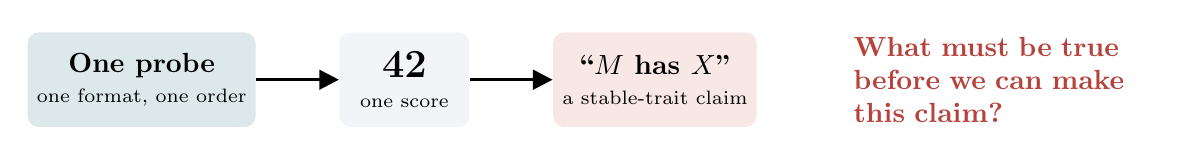
\begin{tikzpicture}[x=1cm,y=1cm]
    \node[rounded corners=4pt,draw=none,fill=blueLite,minimum width=2.2cm,
          minimum height=1.2cm,align=center] (probe) {\textbf{One probe}\\[-1pt]\scriptsize one format, one order};
    \node[rounded corners=4pt,draw=none,fill=softgray,minimum width=1.65cm,
          minimum height=1.2cm,right=1.05cm of probe,align=center] (score)
          {{\Large\bfseries 42}\\[-1pt]\scriptsize one score};
    \node[rounded corners=4pt,draw=none,fill=redLite,minimum width=2.25cm,
          minimum height=1.2cm,right=1.05cm of score,align=center] (claim)
          {\textbf{``$M$ has $X$''}\\[-1pt]\scriptsize a stable-trait claim};
    \draw[-{Triangle[length=2.5mm]},line width=1.2pt] (probe)--(score);
    \draw[-{Triangle[length=2.5mm]},line width=1.2pt] (score)--(claim);
    \node[right=1.1cm of claim,align=left,text width=3.9cm] {\color{red}\bfseries
      What must be true\\before we can make\\this claim?};
  \end{tikzpicture}
  \vfill
  {\small\presenter\quad\textcolor{muted}{|}\quad\affiliation\quad\textcolor{muted}{|}\quad\conference}
\end{frame}

\begin{frame}{The motivating puzzle: the conclusion can move while the task stays fixed}
  \vspace{0.1cm}
  \begin{columns}[T,onlytextwidth]
    \column{0.53\textwidth}
      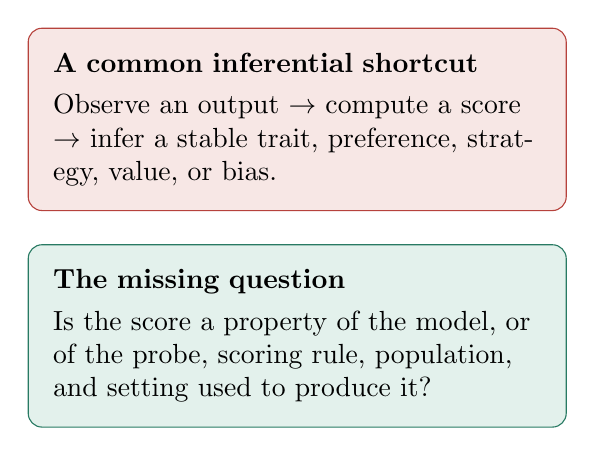
\begin{tikzpicture}
        \node[rounded corners=5pt,draw=red,fill=redLite,text width=6.2cm,
              align=left,inner sep=9pt] {
          \textbf{A common inferential shortcut}\par\vspace{3pt}
          Observe an output $\rightarrow$ compute a score $\rightarrow$
          infer a stable trait, preference, strategy, value, or bias.};
        \node[below=0.42cm of current bounding box.south,anchor=north,
              rounded corners=5pt,draw=green,fill=greenLite,text width=6.2cm,
              align=left,inner sep=9pt] {
          \textbf{The missing question}\par\vspace{3pt}
          Is the score a property of the model, or of the probe, scoring rule,
          population, and setting used to produce it?};
      \end{tikzpicture}
    \column{0.43\textwidth}
      \vspace{0.05cm}
      \bigstat{red}{76 points}{accuracy movement after a format change}\par\vspace{0.45cm}
      \bigstat{red}{82.5\%}{one pairwise-judge comparison flipped by order}\par\vspace{0.45cm}
      \bigstat{amber}{95\% $\to$ 16\%}{cooperation changed across model variants in one game}
  \end{columns}
  \source{Sclar et al. (2024); Wang et al. (2024); Li and Shirado (2025). These are documented extreme settings, not prevalence estimates.}
\end{frame}

\begin{frame}{Our thesis: behavioural evaluation is a measurement problem}
  \centering
  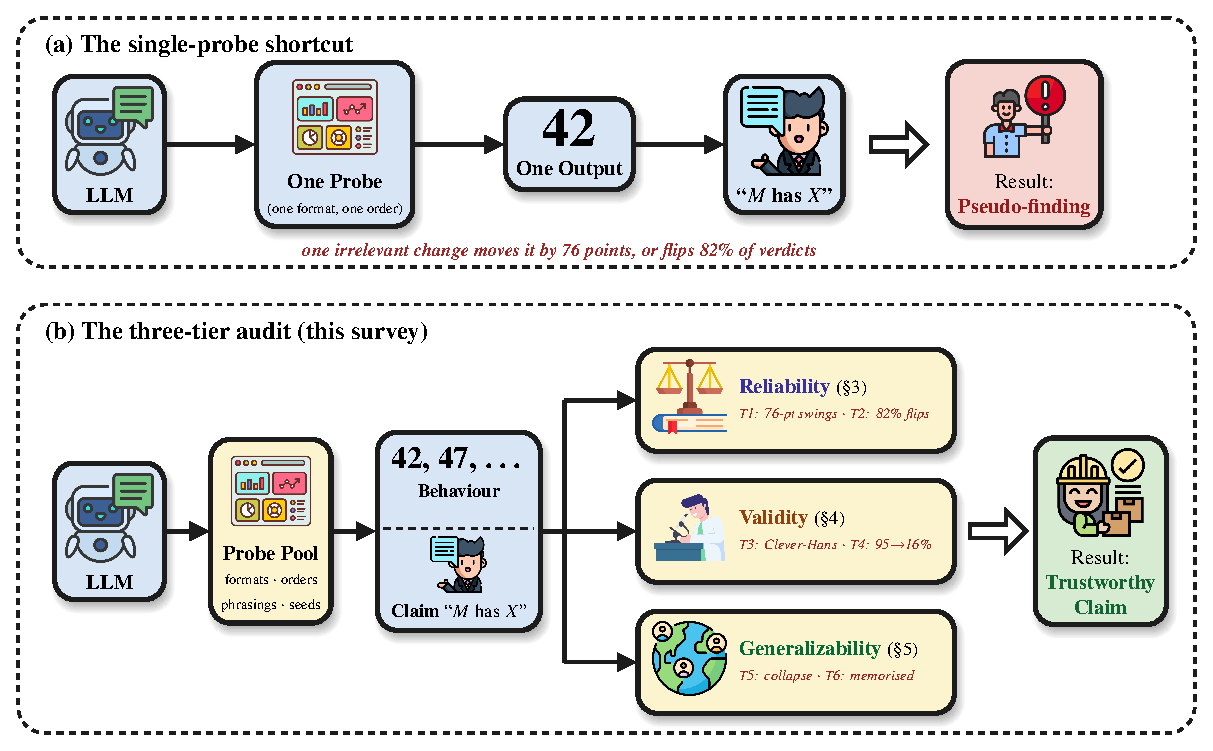
\includegraphics[width=0.93\textwidth,height=0.72\textheight,keepaspectratio]{../figures/core/tikz_hero.pdf}
  \par\vspace{-0.18cm}
  {\small\color{navy}\bfseries The contribution is the audit between observation and interpretation.\par}
\end{frame}

\begin{frame}{One pipeline, three questions}
  \vspace{0.15cm}
  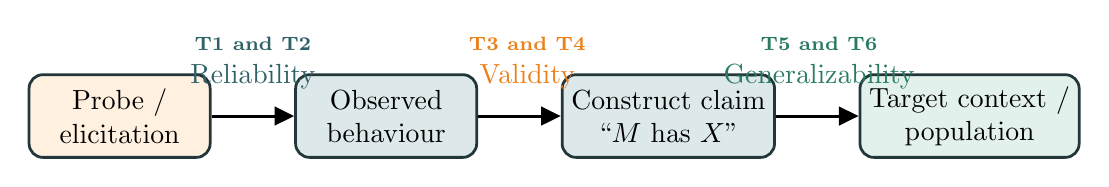
\begin{tikzpicture}[node distance=1.05cm,
    box/.style={rounded corners=5pt,draw=navy,line width=1pt,fill=white,
      minimum width=2.3cm,minimum height=1.05cm,align=center},
    arr/.style={-{Triangle[length=2.5mm]},line width=1.1pt}]
    \node[box,fill=amberLite] (p) {Probe /\\elicitation};
    \node[box,right=of p,fill=blueLite] (o) {Observed\\behaviour};
    \node[box,right=of o,fill=blueLite] (c) {Construct claim\\``$M$ has $X$''};
    \node[box,right=of c,fill=greenLite] (d) {Target context /\\population};
    \draw[arr] (p)--(o); \draw[arr] (o)--(c); \draw[arr] (c)--(d);
    \node[above=0.22cm of $(p)!0.5!(o)$,text=blue,align=center]
      {\scriptsize\bfseries T1 and T2\\Reliability};
    \node[above=0.22cm of $(o)!0.5!(c)$,text=amber,align=center]
      {\scriptsize\bfseries T3 and T4\\Validity};
    \node[above=0.22cm of $(c)!0.5!(d)$,text=green,align=center]
      {\scriptsize\bfseries T5 and T6\\Generalizability};
  \end{tikzpicture}
  \vspace{0.55cm}
  \begin{columns}[T,onlytextwidth]
    \column{0.32\textwidth}\centering
      \textbf{Does the number hold still?}\par
      \small under irrelevant probe changes
    \column{0.32\textwidth}\centering
      \textbf{Does it measure $X$?}\par
      \small rather than a shortcut or scoring choice
    \column{0.32\textwidth}\centering
      \textbf{Does the claim transfer?}\par
      \small beyond the tested sample and setting
  \end{columns}
\end{frame}

\begin{frame}{The survey reorganises a fragmented literature into six threats}
  \centering
  \begin{columns}[T,onlytextwidth]
    \column{0.325\textwidth}
      \tierbox{blue}{blueLite}{Tier 1: Reliability}{T1 Prompt \& format\\[3pt]T2 Order \& position}
    \column{0.325\textwidth}
      \tierbox{amber}{amberLite}{Tier 2: Validity}{T3 Construct validity\\[3pt]T4 Benchmark validity}
    \column{0.325\textwidth}
      \tierbox{green}{greenLite}{Tier 3: Generalizability}{T5 Population \& aggregation\\[3pt]T6 Ecology \& leakage}
  \end{columns}
  \vspace{0.55cm}
  
\begin{tikzpicture}
    \node[rounded corners=5pt,fill=navy,text=white,text width=11.7cm,
          align=center,inner sep=8pt] {\bfseries
      Same failure modes, different names: machine psychology, strategic games,
      social simulation, and LLM-as-a-judge.};
  \end{tikzpicture}
  \source{Structured narrative review of 278 cited records; selection and scope protocol reported in the appendix.}
\end{frame}

\begin{frame}{Tier 1: a stable-looking score can be a property of the probe}
  \begin{columns}[T,onlytextwidth]
    \column{0.47\textwidth}
      \claimbox{blue}{\textbf{T1: Prompt \& format}\par
        Equivalent formats, punctuation, wording, or decoding choices can change
        measured performance.}\par\vspace{0.3cm}
      \claimbox{blue}{\textbf{T2: Order \& position}\par
        Models and judges can prefer a slot, label, or earlier answer independently
        of content.}
    \column{0.49\textwidth}
      \resizebox{\linewidth}{!}{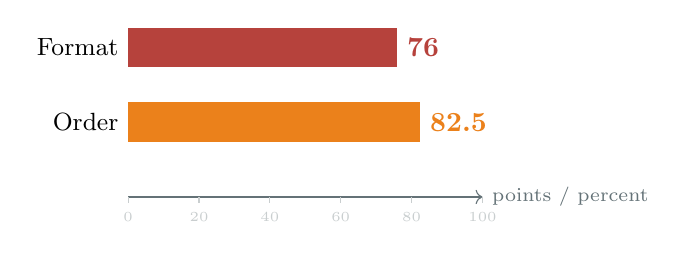
\begin{tikzpicture}[x=0.045cm,y=1cm]
        \draw[->,muted] (0,0)--(100,0) node[right]{\scriptsize points / percent};
        \fill[red] (0,1.65) rectangle (76,2.15);
        \node[left] at (0,1.90){\small Format};
        \node[right,text=red] at (76,1.90){\bfseries 76};
        \fill[amber] (0,0.70) rectangle (82.5,1.20);
        \node[left] at (0,0.95){\small Order};
        \node[right,text=amber] at (82.5,0.95){\bfseries 82.5};
        \foreach \x in {0,20,40,60,80,100}{\draw[muted!35] (\x,0)--(\x,-.08) node[below]{\tiny\x};}
      \end{tikzpicture}}
      \vspace{0.55cm}
      \textbf{Takeaway}\par
      One probe estimates one conditional response. It does not identify a
      stable model property without a declared probe pool.
  \end{columns}
  \source{Sclar et al. (2024); Wang et al. (2024); Dominguez-Olmedo et al. (2024).}
\end{frame}

\begin{frame}{Tier 2: even a stable number may measure the wrong thing}
  \begin{columns}[T,onlytextwidth]
    \column{0.48\textwidth}
      \textbf{Construct validity (T3)}
      \begin{itemize}\setlength\itemsep{0.28cm}
        \item Human questionnaires do not automatically retain their meaning on models.
        \item Response style can be recorded as personality or value variance.
        \item Across 56 models, \alert{81 to 90\%} of profile variation was directional response bias.
      \end{itemize}
    \column{0.48\textwidth}
      \textbf{Normative-benchmark validity (T4)}
      \begin{itemize}\setlength\itemsep{0.28cm}
        \item ``Strategic'', ``rational'', ``human-like'', and ``coherent'' are different targets.
        \item A model may violate equilibrium play while satisfying consistent-choice axioms.
        \item Reporting the scoring rule fixes what the result means.
      \end{itemize}
  \end{columns}
  \vspace{0.4cm}
  \resizebox{0.85\textwidth}{!}{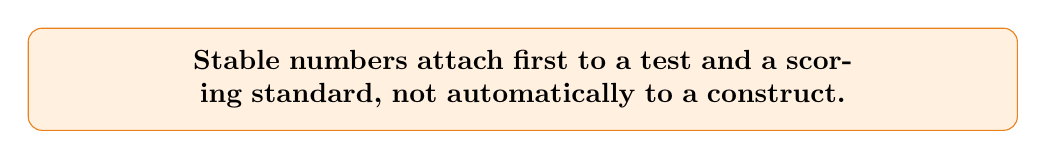
\begin{tikzpicture}
    \node[rounded corners=5pt,draw=amber,fill=amberLite,text width=12cm,
      align=center,inner sep=8pt]{\bfseries Stable numbers attach first to a test and a scoring standard, not automatically to a construct.};
  \end{tikzpicture}}
  \source{Gupta et al. (2024); Shu et al. (2024); Meyer et al. (2026); Akata et al. (2025); Chen et al. (2023).}
\end{frame}

\begin{frame}{Tier 3: when the probe does not resemble deployment}
  \begin{columns}[T,onlytextwidth]
    \column{0.32\textwidth}\centering
      {\Large\bfseries\color{green}$>0.99$}\par
      \small probability on one modal opinion after distribution collapse\par
      \vspace{0.3cm}\scriptsize OpinionQA
    \column{0.32\textwidth}\centering
      {\Large\bfseries\color{green}50.5\% / 22.8\%}\par
      \small strongest model mean / hardest split under information asymmetry\par
      \vspace{0.3cm}\scriptsize InformativeBench
    \column{0.32\textwidth}\centering
      {\Large\bfseries\color{green}7\% $\to$ 80\%}\par
      \small welfare after a payoff rewrite in one social-dilemma setting\par
      \vspace{0.3cm}\scriptsize CoopEval
  \end{columns}
  \vspace{0.55cm}
  \begin{columns}[T,onlytextwidth]
    \column{0.48\textwidth}
      \textbf{T5: population \& aggregation}\par
      \small Means can flatten subgroups, interactions, and human variability.
    \column{0.48\textwidth}
      \textbf{T6: ecology \& leakage}\par
      \small Canonical or memorised probes can overstate transfer to deployment.
  \end{columns}
  \source{Santurkar et al. (2023); Liu et al. (2024); Tewolde et al. (2026). Each magnitude is tied to its reported setting.}
\end{frame}

\begin{frame}{Contribution 2: quantify fragility relative to signal}
  \begin{columns}[c,onlytextwidth]
    \column{0.52\textwidth}
      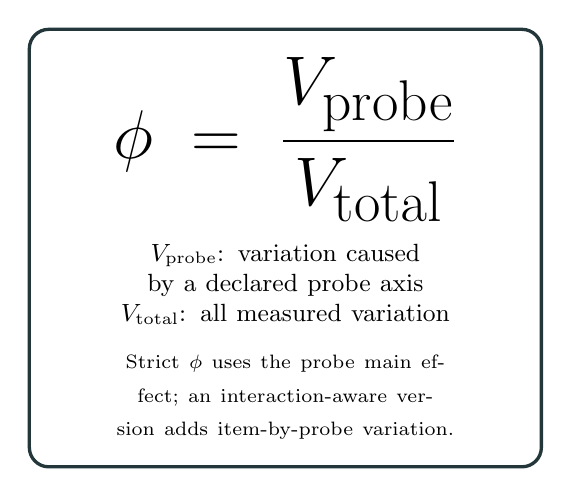
\begin{tikzpicture}
        \node[rounded corners=7pt,draw=navy,line width=1.2pt,fill=white,
          text width=5.8cm,align=center,inner sep=10pt] {
          {\Huge\bfseries $\displaystyle \phi=\frac{V_{\rm probe}}{V_{\rm total}}$}\par\vspace{7pt}
          \small $V_{\rm probe}$: variation caused by a declared probe axis\par
          $V_{\rm total}$: all measured variation\par\vspace{5pt}
          \scriptsize Strict $\phi$ uses the probe main effect; an interaction-aware
          version adds item-by-probe variation.};
      \end{tikzpicture}
    \column{0.44\textwidth}
      \textbf{Why not report sensitivity alone?}
      \begin{itemize}\setlength\itemsep{0.25cm}
        \item The same prompt movement matters differently when model separation is large or tiny.
        \item $\phi$ is claim-, model-, and axis-specific.
        \item It converts stability into a design question: how many probes are needed?
      \end{itemize}
  \end{columns}
  \vspace{0.35cm}
  {\centering\color{red}\bfseries A small $\phi$ validates only the declared axis, not the construct.\par}
\end{frame}

\begin{frame}{Matched comparison: the tested axis accounts for 11$\times$ more variation}
  \begin{columns}[c,onlytextwidth]
    \column{0.47\textwidth}
      \resizebox{\linewidth}{!}{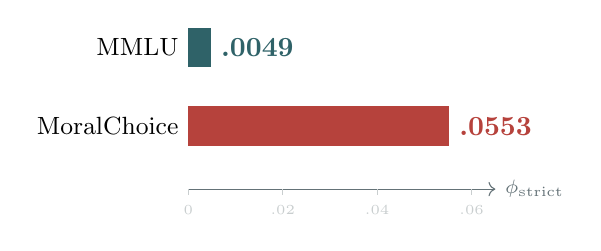
\begin{tikzpicture}[x=60cm,y=1cm]
        \draw[->,muted] (0,0)--(.065,0) node[right]{\scriptsize $\phi_{\rm strict}$};
        \fill[blue] (0,1.55) rectangle (.0049,2.05);
        \node[left] at (0,1.80){\small MMLU};
        \node[right,text=blue] at (.0049,1.80){\bfseries .0049};
        \fill[red] (0,0.55) rectangle (.0553,1.05);
        \node[left] at (0,0.80){\small MoralChoice};
        \node[right,text=red] at (.0553,0.80){\bfseries .0553};
        \foreach \x in {0,.02,.04,.06}{\draw[muted!35] (\x,0)--(\x,-.08) node[below]{\tiny\x};}
      \end{tikzpicture}}
    \column{0.49\textwidth}
      \textbf{Matched design}
      \begin{itemize}\setlength\itemsep{0.27cm}
        \item Item-level analysis with difficulty matching.
        \item Same estimator, explicit probe axis.
        \item Eleven-fold contrast between these measurements.
      \end{itemize}
      \vspace{0.25cm}
      \alert{Not supported:} ``behaviour is generally eleven times more fragile than capability.''
  \end{columns}
  \vspace{0.35cm}
  \resizebox{0.85\textwidth}{!}{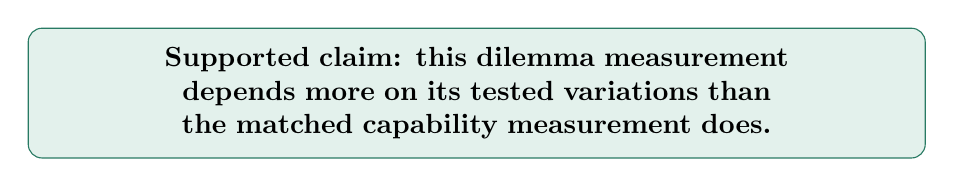
\begin{tikzpicture}
    \node[rounded corners=5pt,fill=greenLite,draw=green,text width=10.9cm,align=center,inner sep=7pt]
      {\bfseries Supported claim: this dilemma measurement depends more on its tested variations than the matched capability measurement does.};
  \end{tikzpicture}}
\end{frame}

\begin{frame}{We tried to falsify our own headline}
  \begin{columns}[T,onlytextwidth]
    \column{0.31\textwidth}
      \equalclaimbox{green}{\textbf{Positive control}\par
        A behavioural positive control with a strong expected preference has
        median $\phi_{\rm strict}=0.0005$ under language variation.}\par
      \vspace{0.18cm}{\scriptsize Behaviour is not inherently fragile.}
    \column{0.31\textwidth}
      \equalclaimbox{amber}{\textbf{Axis dependence}\par
        The same control reaches $\phi=0.30$ when presentation order is added.}\par
      \vspace{0.18cm}{\scriptsize Robustness on one axis does not transfer to another.}
    \column{0.31\textwidth}
      \equalclaimbox{blue}{\textbf{Ceiling check}\par
        Easy capability items have little binary variance left to move.}\par
      \vspace{0.18cm}{\scriptsize Some apparent robustness is arithmetic, not substantive.}
  \end{columns}
  \vspace{0.5cm}
  {\centering\Large\bfseries\color{navy}Fragility depends on three things\\[2pt]
  \textcolor{red}{(claim, probe axis, model)}.\par}
\end{frame}

\begin{frame}{Uncertainty changes what we are allowed to say}
  \begin{columns}[c,onlytextwidth]
    \column{0.49\textwidth}
      \centering
      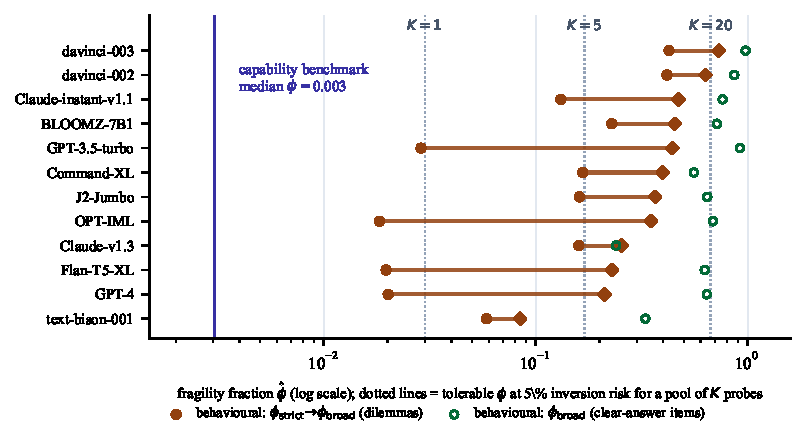
\includegraphics[width=0.95\linewidth,height=0.60\textheight,keepaspectratio]{../figures/core/phi_forest.pdf}
    \column{0.47\textwidth}
      \bigstat{amber}{.034 $\to$ .172}{median interval width after resampling probes as well as items}
      \vspace{0.55cm}
      \bigstat{red}{3 / 66}{model pairs that remain separated under the paired bootstrap}
      \vspace{0.55cm}
      \textbf{Implication}\par
      \small Point rankings are descriptive. Pairwise superiority claims need paired uncertainty over the probe pool.
  \end{columns}
\end{frame}

\begin{frame}{The metric leads directly to a better intervention}
  \begin{columns}[c,onlytextwidth]
    \column{0.48\textwidth}
      \resizebox{\linewidth}{!}{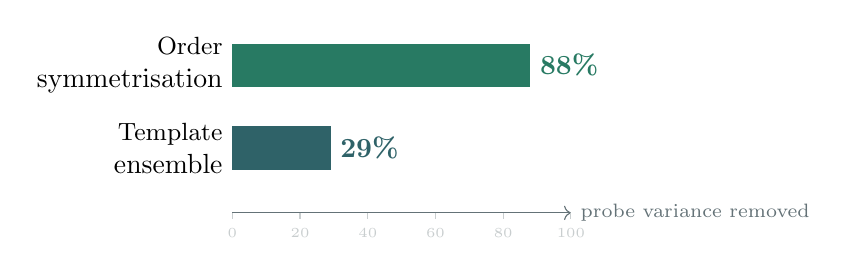
\begin{tikzpicture}[x=0.043cm,y=1cm]
        \draw[->,muted] (0,0)--(100,0) node[right]{\scriptsize probe variance removed};
        \fill[green] (0,1.6) rectangle (88,2.15);
        \node[left,align=right] at (0,1.88){\small Order\\symmetrisation};
        \node[right,text=green] at (88,1.88){\bfseries 88\%};
        \fill[blue] (0,.55) rectangle (29,1.10);
        \node[left,align=right] at (0,.82){\small Template\\ensemble};
        \node[right,text=blue] at (29,.82){\bfseries 29\%};
        \foreach \x in {0,20,40,60,80,100}{\draw[muted!35] (\x,0)--(\x,-.08) node[below]{\tiny\x};}
      \end{tikzpicture}}
    \column{0.48\textwidth}
      \textbf{A practical rule}
      \begin{enumerate}\setlength\itemsep{0.28cm}
        \item Decompose variation by probe axis.
        \item Target the term that carries the variance.
        \item Re-estimate uncertainty after mitigation.
      \end{enumerate}
      \vspace{0.25cm}
      \small On clear-answer items, the ordering reverses. The best remedy is empirical, not universal.
  \end{columns}
  \vspace{0.55cm}
  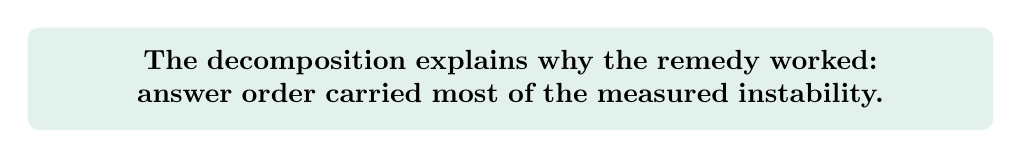
\begin{tikzpicture}
    \node[rounded corners=4pt,draw=none,fill=greenLite,
      text width=11.7cm,align=center,inner sep=8pt]
      {\bfseries The decomposition explains why the remedy worked:\\
      answer order carried most of the measured instability.};
  \end{tikzpicture}
\end{frame}

\begin{frame}{End-to-end audit: what can we still claim?}
  \begin{columns}[T,onlytextwidth]
    \column{0.48\textwidth}
      \claimbox{red}{\textbf{Claim that weakens}\par
        ``The model has a stable personality profile.''\par\vspace{3pt}
        Equivalent prompts move scores; response style dominates between-model
        variance; self-report weakly predicts open-ended behaviour.}
    \column{0.48\textwidth}
      \claimbox{green}{\textbf{Comparative claim that survives}\par
        On the tested dilemma probes, GPT-4 is less probe-dependent than the other
        eleven models.\par\vspace{3pt}
        The claim is relational and explicitly scoped to the probe pool.}
  \end{columns}
  \vspace{0.45cm}
  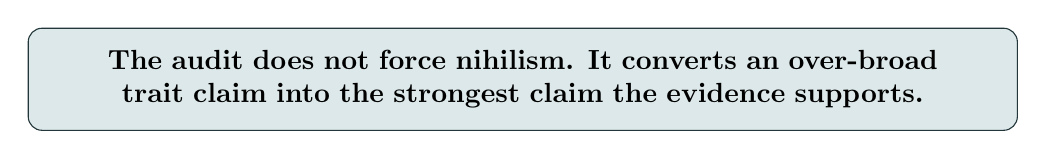
\begin{tikzpicture}
    \node[rounded corners=5pt,draw=navy,fill=blueLite,text width=12cm,align=center,inner sep=8pt]
      {\bfseries The audit does not force nihilism. It converts an over-broad trait claim into the strongest claim the evidence supports.};
  \end{tikzpicture}
\end{frame}

\begin{frame}{A checklist authors and reviewers can run}
  \begin{columns}[T,onlytextwidth]
    \column{0.48\textwidth}
      \textbf{Design}
      \begin{enumerate}\setlength\itemsep{0.20cm}
        \item Name the construct and target context.
        \item Declare a probe pool and expected invariances.
        \item Balance order; vary formats, wording, and seeds.
        \item Include an ecological or subgroup stress test.
      \end{enumerate}
    \column{0.48\textwidth}
      \textbf{Analysis \& reporting}
      \begin{enumerate}\setlength\itemsep{0.20cm}
        \setcounter{enumi}{4}
        \item Decompose model, item, probe, and interaction variance.
        \item Bootstrap items and probes together.
        \item Validate the test and state the scoring standard.
        \item Report the claim with its tested scope.
      \end{enumerate}
  \end{columns}
  \vspace{0.38cm}
  {\centering\color{navy}\bfseries Release probe-level outcomes: without them, fragility cannot be re-audited.\par}
\end{frame}

\begin{frame}{What changes if the field adopts this view?}
  \begin{columns}[T,onlytextwidth]
    \column{0.31\textwidth}
      \tierbox{blue}{blueLite}{For benchmark builders}{A benchmark becomes a sampled measurement design, not a single prompt template.}
    \column{0.31\textwidth}
      \tierbox{amber}{amberLite}{For reviewers}{Ask which link supports the claim, which axis was varied, and what remains invariant.}
    \column{0.31\textwidth}
      \tierbox{green}{greenLite}{For deployment}{Prefer scoped comparative claims over essentialist statements about what a model ``is''.}
  \end{columns}
  \vspace{0.55cm}
  
\begin{tikzpicture}
    \node[rounded corners=5pt,fill=navy,text=white,text width=11.8cm,align=center,inner sep=9pt]
      {\Large\bfseries Impact = fewer pseudo-findings, clearer scopes,\\and interventions targeted at measured failure modes.};
  \end{tikzpicture}
\end{frame}

\begin{frame}{Take-home message}
  \vspace{0.25cm}
  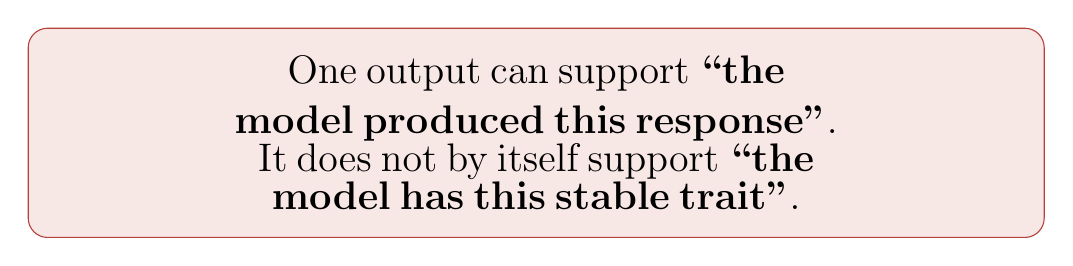
\begin{tikzpicture}
    \node[rounded corners=7pt,draw=red,fill=redLite,text width=12.2cm,align=center,inner sep=10pt]
      {\Large One output can support \textbf{``the model produced this response''}.\\It does not by itself support \textbf{``the model has this stable trait''}.};
  \end{tikzpicture}
  \vspace{0.5cm}
  \begin{columns}[T,onlytextwidth]
    \column{0.31\textwidth}\centering
      {\large\bfseries\color{blue}1. Audit the link}\par\small reliability $\to$ validity $\to$ transfer
    \column{0.31\textwidth}\centering
      {\large\bfseries\color{amber}2. Measure fragility}\par\small relative to the signal and named axis
    \column{0.31\textwidth}\centering
      {\large\bfseries\color{green}3. Scope the claim}\par\small say exactly what survives the audit
  \end{columns}
  \vfill
  {\centering\small\color{muted}Questions? \quad Repository / QR code placeholder: \texttt{anonymous-url}\par}
\end{frame}

% Backup slides
\appendix

\begin{frame}{Backup: review scope and evidence policy}
  \begin{itemize}\setlength\itemsep{0.28cm}
    \item Structured narrative review, not a PRISMA systematic review.
    \item 278 cited records across games, social simulation, machine psychology,
          and LLM-as-a-judge.
    \item Headline magnitudes are tagged by role: extreme stress test, broad
          evidence, mechanism, or mitigation.
    \item Preprints support the map but do not carry a threat's headline alone.
    \item Main evidence is densest in forced-choice English text; multilingual,
          multimodal, and open-ended evidence extends the taxonomy without proving
          that every threat grows outside that setting.
  \end{itemize}
\end{frame}

\begin{frame}{Backup: variance decomposition behind \texorpdfstring{$\phi$}{phi}}
  \small
  For one model, outcome $y_{ik}$ on item $i$ under test variant $k$ is
  \[
    y_{ik}=\mu+a_i+b_k+(ab)_{ik}+\varepsilon_{ik}.
  \]
  The strict version counts only the shared probe shift. The broad version also
  counts cases where the same probe helps some items and hurts others:
  \[
    \phi_{\rm strict}=\frac{\sigma_b^2}{\sigma_{\rm total}^2},
    \qquad
    \phi_{\rm broad}=\frac{\sigma_b^2+\sigma_{ab}^2}{\sigma_{\rm total}^2}.
  \]
  Broad $\phi$ requires repeated observations to separate interaction from
  run-to-run noise. With one binary observation per cell, only strict $\phi$ is
  identifiable.
  \vspace{0.35cm}
  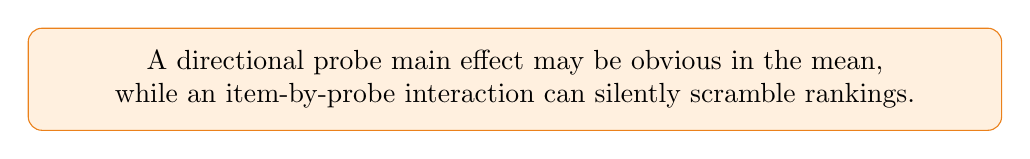
\begin{tikzpicture}
    \node[rounded corners=5pt,draw=amber,fill=amberLite,text width=11.8cm,align=center,inner sep=8pt]
      {A directional probe main effect may be obvious in the mean, while an item-by-probe interaction can silently scramble rankings.};
  \end{tikzpicture}
\end{frame}

\begin{frame}{Backup: using \texorpdfstring{$\phi$}{phi} to size the probe pool}
  \begin{columns}[c,onlytextwidth]
    \column{0.48\textwidth}
      \small Probe noise is shared within a probe and therefore is not averaged
      away by adding more items or samples. More independent probes are required.
      At 5\% accepted inversion risk in the MoralChoice-anchored independence case:
    \column{0.48\textwidth}
      \centering
      \begin{tabular}{cc}
        \toprule
        Probe count $K$ & Permitted $\phi$ \\
        \midrule
        1  & 0.03 \\
        5  & 0.17 \\
        10 & 0.34 \\
        20 & 0.67 \\
        \bottomrule
      \end{tabular}
  \end{columns}
  \vspace{0.45cm}
  \centering\bfseries A universal cutoff is not meaningful without $K$, the model gap, and an accepted error rate.
\end{frame}

\begin{frame}{Backup: remedy cost and what each intervention buys}
  \small
  \begin{tabularx}{\textwidth}{>{\bfseries\raggedright\arraybackslash}p{3.0cm}>{\raggedright\arraybackslash}X>{\raggedright\arraybackslash}p{3.2cm}}
    \toprule
    Remedy & What it addresses & Main cost \\
    \midrule
    Balanced permutation & Signed order / position effects & $2\times$ for pairwise judging \\
    Probe or template pool & Format, wording, seed variation & Linear in pool size $K$ \\
    Variance decomposition & Locates the dominant axis & No new inference if outcomes retained \\
    Gold-slice calibration & Corrects surrogate labels; returns coverage & Human-labelled subset \\
    Ecological stress test & Measures transfer rather than assuming it & Task-specific environment \\
    \bottomrule
  \end{tabularx}
\end{frame}

\begin{frame}{Backup: sources for headline examples}
  \footnotesize
  \begin{tabularx}{\textwidth}{p{3.0cm}X}
    \toprule
    Example & Primary source \\
    \midrule
    76-point format swing & Sclar et al. (2024), \emph{Quantifying Language Models' Sensitivity to Spurious Features in Prompt Design} \\
    82.5\% order conflict & Wang et al. (2024), \emph{Large Language Models are not Fair Evaluators} \\
    Opinion distributions & Santurkar et al. (2023), \emph{Whose Opinions Do Language Models Reflect?} \\
    Information asymmetry & Liu et al. (2024), \emph{Autonomous Agents for Collaborative Task under Information Asymmetry} \\
    Cooperation rewrite & Tewolde et al. (2026), \emph{CoopEval} \\
    Response-style variance & Meyer et al. (2026), \emph{Apparent Personality in Language Models} \\
    \bottomrule
  \end{tabularx}
\end{frame}

\end{document}
